\chapter{Data Analysis}
\label{ch:data_analysis}
The work discussed in this chapter was done in close collaboration with Dr. Ralf
Seidl, Dr. Francesca Giordano, Daniel Jumper, and Abraham Meles. Eventually the
analysis group merged with another year's analysis group, bringing in Dr. Sanghwa
Park, and Dr. Chong Kim, who have made crucial contributions to this analysis,
and have studied the complimentary 2012 data set, producing their own PhD theses
on this analysis. Dr. Hideyuki Oide has also heavily influenced the techniques
and work-flow of this analysis, pioneering many of the techniques used here (at
PHENIX at least) for his analysis of the 2011 data set.

\label{ch:data_collection}
\section{Overview}
Although we have discussed in detail the theoretical motivations for the W
physics program, as well as the machines producing the necessary collisions and
recording data produced from these collisions, we have not yet addressed the
form of the data set itself, and the substantial engineering it takes to extract
the signal of interest out of that data set.

The relative abundance of the $p + p \rightarrow W^\pm \rightarrow \mu^\pm +
\nu$ signal events is rather low, compared to the other interactions which may
take place when two protons collide. We must allow several hundred million
proton proton collisions to occur, before we have a high probability of
observing just one W-Boson event. 

We discussed in the previous chapter how careful triggering is employed in order
to ensure that any time this event does occur, it is recorded. This does not
guarantee that we \textit{only} record these events. Background events are still
recored much more frequently than signal events, even with the improved
triggering. The number of $W\rightarrow\mu$ events produced over the 2013 data
set number in the hundreds, while the total number of recorded events is
approximately 15 billion.

This leads to the substantial problem of fishing out the appropriate physics
events from the 15 billion event haystack. Why, I hear you ask, don't we just
have a detector which can record only the W-Boson events of interest?

Because, as a multipurpose spectrometer, PHENIX must be ready to take
all kinds of data, and satisfy many experimental requirements, in addition to
fitting a lot of functionality into a relatively tight budget, as is common for
federally funded research. Although this measurement would have been made
much simpler with a forward calorimeter, we can't simply build and install a
calorimeter the moment that an analysis would benefit from its presence.

So, instead, we must rely on our ingenuity and deep understanding of the data
set, to tease out the results we want to measure.

\section{Raw Data to Reconstructed Parameters}

Any time a PHENIX trigger condition is satisfied, all of the information
recorded by the PHENIX spectrometer are read out from temporary on-detector
memory, and fed into a data stream that eventually is archived as a `PHENIX Raw
Data File Format' or PRDFF. 

PRDFF data is hierarchical, first being organized by event-type, and
then organized by packet-type.  There are many event types--`DATAEVENTS'
typically carry the information relevant to a physics analysis, whereas other
event-types carry very important QA information for determining the status of
the RHIC apparatus, the beam, polarization, and PHENIX performance.

Every packet has a header, which contains general information such as what the
packet contains, and in what order that packet was received. Every packet
recorded can be associated with a unique event-sequence number, which specifies
roughly the order in which the event owning the packet was received by the DAQ.
Within a given run number, an event-number is guaranteed to be unique. The
complexity of the packet is limited by the bandwidth available to move data off
PHENIX onto other storage, and the buffers/reconstruction ability of the front
end electronics modules built onto PHENIX subsystems. PHENIX archives data from
the DAQ at a rate of approximately 700 Megabytes per second--or one compact
disk.

Generally, raw PHENIX data is too complex to use straight-away, because minimal
to no reconstruction of physical properties for a certain event is done, due to
hardware limitations and time limitations--some of this raw data is often
directly used in triggering decisions, which must be made once every 106
nanoseconds or faster (the bunch crossing frequency).

The raw data collected from PHENIX undergoes a process called ``Data Production'',
where physical parameters are reconstructed from the simpler raw data. Raw data
could take any form--for example--which cathode strips were activated in an
event in the muon tracker, or, the number of photons counted in a
photomultiplier tube. This information is often combined with extensive survey
information about the geometry of a given detector, the known magnetic field in
a detector, to reconstruct quantities such as momentum, or deposited energy.

Once reconstruction has finished in a Data Production, the data are then
repackaged into ROOT files, often times internally structured into custom output
objects which are associated with a various detector. These output objects are
simply custom written C++ classes which have a serialization scheme, which have
libraries and dictionaries compiled that allow for them to be serialized into
ROOT's file format.

For the purposes of this analysis, all data has been reconstructed and
serialized into a specific type of output object called a `picoDST' or even more
concisely, `pDST'. This name, like many others in PHENIX has historical context:
DST stands for `Data Summary Tape' hearkening back to the days when data was
stored primarily on magnetic tape (it is still archived on magnetic tape!), and
`pico' because of its relatively small disk-space requirement, compared to
`nanoDST' files or simply `DST' files. I'm not making this up, I swear!

\section{Choosing Analysis Variables}

Even data reduced to the point of a pDST still is much more complicated and
comprehensive than what is needed for this analysis--there are thousands of
variables relating to reconstruction parameters. We only need a handful of
variables for this analysis, summarized on Tables
\ref{tab:evt_variables},\ref{tab:mutr_variables}, \ref{tab:fvtx_variables} and
\ref{tab:rpc_variables}. When Cartesian coordinates are referenced, implicitly,
the reference frame is the PHENIX Coordinate system
(Figure~\ref{fig:phenix_coordinate_system}).

As you can probably guess, the only variables which are truly relevant to this
analysis need to be relevant to understanding two questions:

\begin{enumerate}
  \item \textit{Is this reconstructed muon track the result of a real W-Boson Decay?}
  \item \textit{What is the polarization of the two colliding protons for every recorded collision?}
\end{enumerate}

To properly answer these questions, we need to comprehensively understand what
processes are capable of producing muons, as well as whether or not our detector
can be `tricked' by signals which look like muons, but really aren't. Secondly,
we need a means of recovering the proton spin polarization for each colliding
bunch-pair.

Polarization recovery is straight-forward--we already have mechanisms in the
data stream which number and track the colliding bunch pairs. We additionally
have well defined spin patterns which are applied to the 120 bunches, the same
way every time this pattern is applied to the fill. As discussed previously, we
have good QA apparatuses in place to ensure the advertised spin pattern is the
same as the delivered spin pattern. Since polarization patterns do not typically
change in a standard physics beam fill (if they do, alarms are raised and the
data is typically discarded), all that is needed is to associate a PHENIX run
number, with a RHIC fill number, and then look up the spin pattern, which in
effect, is a database-call. Of course, the overall beam polarization percentage
is an important factor, which dilutes any spin asymmetry, but this is taken into
account in the final spin database QA analysis~\cite{Kim2014}.

This leaves us with the first question, and the difficulty in answering this
question is essentially that it is challenging to differentiate signal
$W\rightarrow\mu$ events from other $X\rightarrow\mu$ events, or even events
which look like muons, but are really due to incorrect track reconstruction.

Therefore, the thrust of the Data Analysis portion of this work is really just
to tease apart the real W-genic muons, from all other muon candidates. To this
requires some substantial feature engineering, and creating some statistical
models, as well as a means of evaluating the performance of these statistical
models--which is difficult because validating any statistical differentiation
technique (aka machine learning technique) requires a labeled data set, and we
intrinsically do not possess this, since otherwise, this analysis would not need
to be done.

\begin{table}
  \centering
  \begin{tabular}{c p{0.6\linewidth}}
      \toprule
      \textbf{Name} & \textbf{Description} \\
      \midrule
      Run\_Number & A unique number identifying a run in a RHIC fill for PHENIX \\
      Evt\_Number & A unique number within a single run identifying the approximate order an event was taken. \\
      Evt\_bbcZ & The event z-vertex calculated by the BBC \\
      triggerbit & The result of a bit-wise `OR' applied to all 32-bit trigger bits which fired \\
      clockcross & The bunch number of the two colliding bunches $[0-119]$. Required to look up the spin polarization, along with Run\_Number \\
      \bottomrule
    \end{tabular}
  \caption{Variables characterizing events overall}
  \label{tab:evt_variables}
\end{table}

\begin{table}
  \centering
  \begin{tabular}{l p{0.8\linewidth}}
    \toprule
    \textbf{Name} & \textbf{(Unit) Description} \\
    \midrule
    Evt\_Nmu & The number of muon tracks reconstructed for a given event \\
    charge & ($\pm e$) The charge associated with a reconstructed muon track \\ 
    $p_z$ & (GeV) The z-momentum associated with the muon track \\
    $p$ & (GeV) The total momentum of a charged track \\
    $\chi^2$ & The result of the Kalman fitter reconstructing the track \\
    lastGap & The last gap in the Muon Tracker which was activated (there are 4) \\
    $\eta$ & The rapidity of the track \\
    $\phi$ & (rad) The azimuthal position angle the track makes relative to the x-axis \\
    DG0 & (cm) A Track matching variable (matching between MuID and MuTR) associated with the MuID road, at MuID station 3. \\
    DDG0 & (degree)  The opening angle between the MuID track road, and the MuTr projection onto the MuID \\
    xSta${}_i$ & (cm) The x-coordinate of the track at Station i,  $i\in{1,2,3}$ of the MuTr \\
    ySta${}_i$ & (cm) The y-coordinate of the track at Station i, $i\in{1,2,3}$ of the MuTr \\

    $\phi_i$ & (rad) The angle the track makes with Station i, $i\in{1,2,3}$, i.e.: $\phi_i = tan^{-1}\left({{x_1}\over{y_i}}\right)$ \\
    $\theta$ & (rad) Azimuthal angle of track, $tan^{-1}\left({p_T \over p_z}\right)$ \\
    DCA${}_z$ & (cm) Distance of closest approach between the z-vertex positions extracted by projecting the MuTR track z-vertex back to the BBC z-vertex \\
    DCA${}_r$ & (cm) Distance of closest approach between the track and beam axis \\ 
    \bottomrule
  \end{tabular}
  \caption{
    Muon tracker variables. Generally, this data set is indexed on a subevent 
    level, where one event will contain all reconstructed muon tracks seen for 
    that event.
  }
  \label{tab:mutr_variables}
\end{table}

\begin{figure}
  \centering
  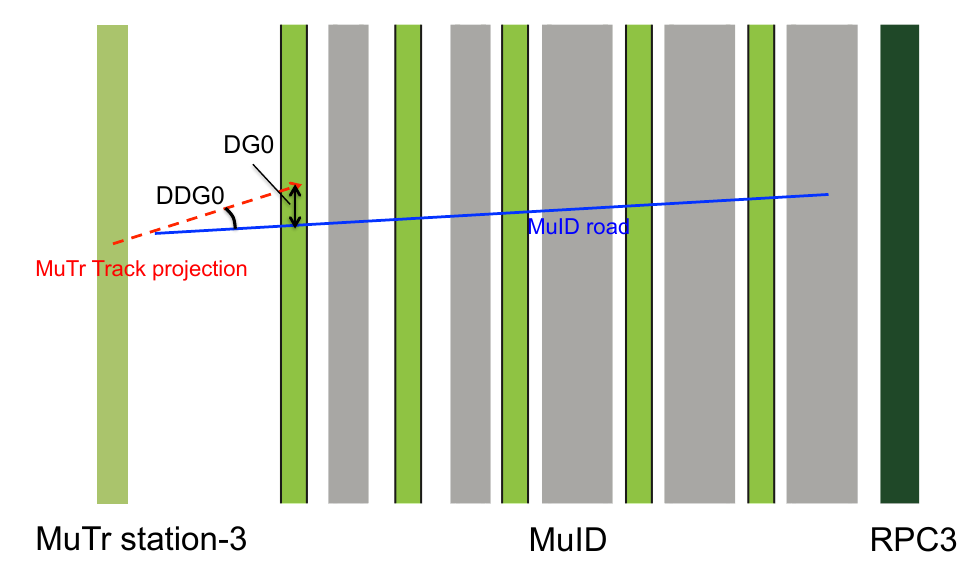
\includegraphics[width=0.7\linewidth]{./figures/dg0_ddg0.png}
  \caption{
    A schematic representation of the matching variables, DG0 and DDG0 at
    the intersection between the Muon Tracker and Muon 
    Identifier~\cite{Oide2012}
  }
  \label{fig:dg0_ddg0}
\end{figure}

\begin{table}
  \centering
  \begin{tabular}{l p{0.7\linewidth}}
    \toprule
    \textbf{Name} & \textbf{Description} \\
    \midrule
    $fvtx_{d\phi}$ & The $\phi$ residual between MuTR track and FVTX track \\
    $fvtx_{d\theta}$ & The $\theta$ residual between the MuTR track and FVTX track \\
    $fvtx_{dr}$ & The radial residual between the MuTR track and the FVTX track \\
    $fvtx_{conebits}$ & The number of FVTX clusters inside a cone around the track defined by: $0.04 rad < dR < 0.52 rad$ where $dR = \sqrt{{d\eta}^2+{d\phi}^2}$\\
    \bottomrule
  \end{tabular}
  \caption{A summary of the variables reconstructed from FVTX raw data~\cite{Meles2015}.}
  \label{tab:fvtx_variables}
\end{table}

\begin{table}
  \centering
  \begin{tabular}{l p{0.7\linewidth}}
    \toprule
    \textbf{Name} & \textbf{Description} \\
    \midrule
    RpcMatchSt1 & Distance of closest approach between projected MuTR track onto the RPC 1 and the closest hit cluster on RPC 1\\
    RpcMatchSt3 & Distance of closest approach between projected MuTR track onto the RPC 3 and the closest hit cluster on RPC 3\\
    \bottomrule
  \end{tabular}
  \caption{RPC Track matching variables}
  \label{tab:rpc_variables}
\end{table}

\begin{figure}
  \centering
  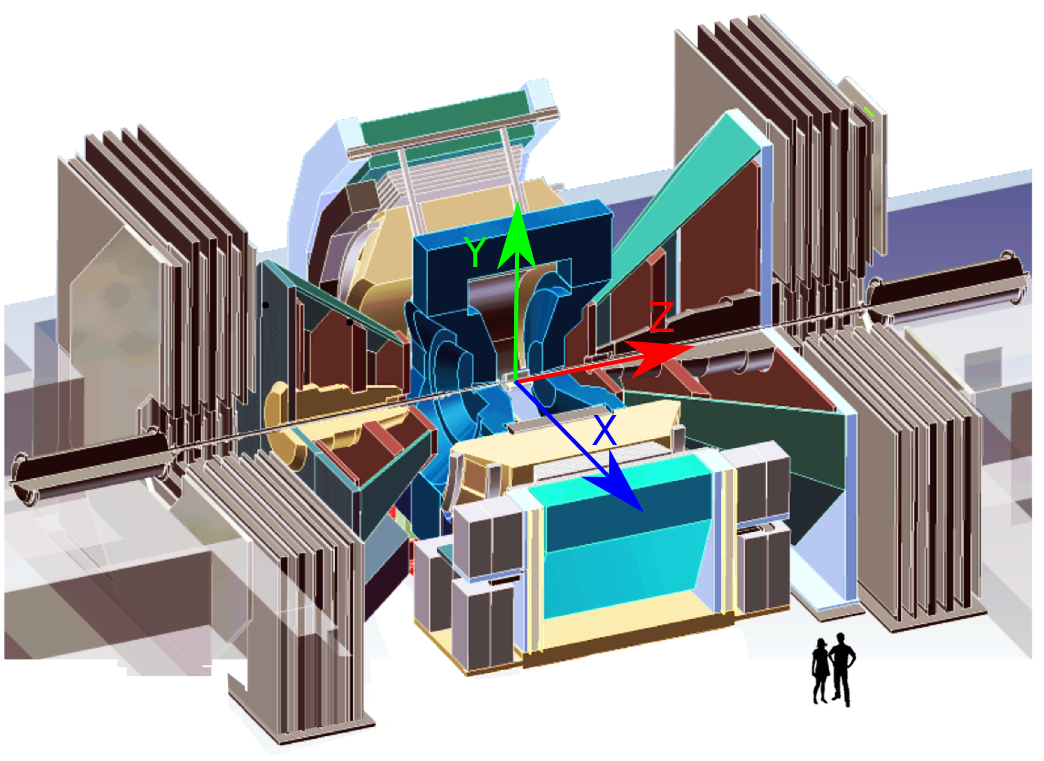
\includegraphics[width=\linewidth]{./figures/phenix_coordinate_system.png}
  \caption{
    The PHENIX coordinate system is shown (RGB arrows) at the center of the
    nominal interaction point within PHENIX, the origin, in this quarter-cutaway
    drawing. The small black figures are actually miniaturized human beings, the
    PHENIX detector is very small--this is a full scale drawing of PHENIX.
    Shown: the x, y, and z coordinates, as well as the azimuthal coordinate,
    $\theta$ and polar coordinate $\phi$ ~\cite{WebPHENIXDrawings}
  }
  \label{fig:phenix_coordinate_system}

\end{figure}


\begin{figure}
  \centering
  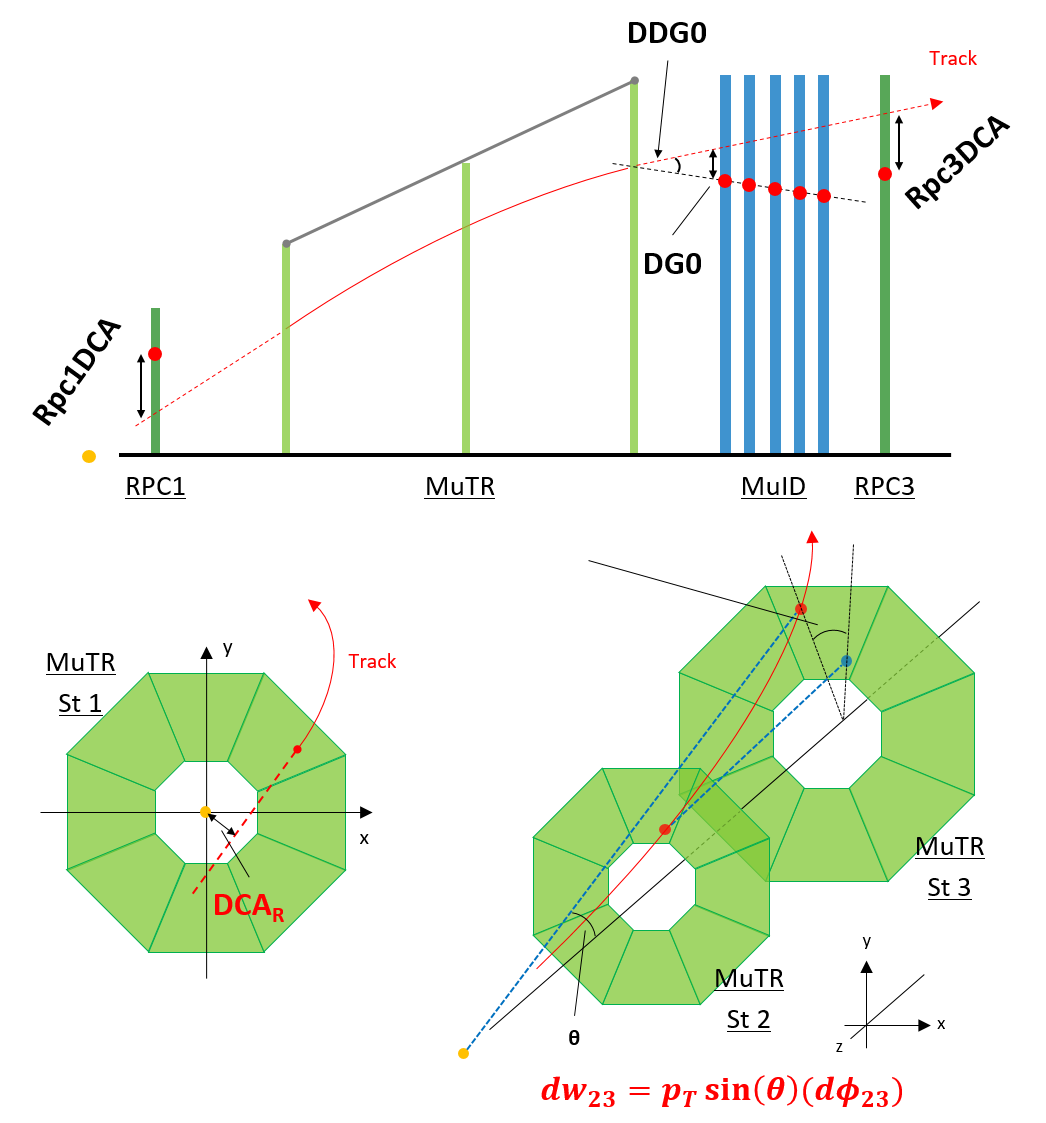
\includegraphics[width=0.8\linewidth]{./figures/kinematic_variables_schematic.png}
  \caption{
    A nice summary of discriminating kinematic variables reproduced with
    permission from Dr. Chong Kim. We see the MuTR tracking planes in green, and
    a muon track penetrating the planes in red, and reference coordinates in the
    lower right-hand corner. The geometric relationship between the roads,
    reconstructed track are shown in the annotations.
  }

\end{figure}

The engineered variables in this analysis are $dw_{13}$, $dw_{23}$,
$d\phi_{13}$, and $d\phi{23}$.  These variables are calculated from
reconstructed physics data. They play an important role in our extraction of the
signal to background ratio.  The $d\phi_{ij}$ variables represent the difference
in azimuthal angle observed at the MuTR station i and j respectively.  $dw_{ij}$
is constructed from $d\phi_{ij}$ as follows:
\begin{equation}
  dw_{ij} = p_T \times sin(\theta) \times d\phi_{ij}
  \label{eq:dw23_definition}
\end{equation}

While $\phi_{i}$ is calculated from the x and y coordinates at Station i:

\begin{equation}
  \phi_i = tan^{-1}\left({ySta_i \over xSta_i}\right)
  \label{eq:phi_definition}
\end{equation}

A common theme amongst these variables is that they should help us distinguish
between high momentum muon tracks from W-Bosons, and other muon tracks. The hope
is that the muon tracks from W-Bosons are kinematically restricted to have a
relatively narrow momentum distribution in the forward kinematic regime, and so
therefore, tracking variables can be used to partially differentiate between
signal and background events.

In general, W-genic events will be mostly straight, geometrically, and so this
constrains the values of variables such as DCA${}_r$ substantially, and other
variables less so. Thus, $dw_{23}$ should be a good discriminator, as it depends
on $p_T$ and the azimuthal bending of the charged tracks, due to the radial
magnetic field in the MuTR.

Our secondary requirement of our variables is that they are relatively
uncorrelated with each-other, to leave plenty of room for statistical modeling.
Ultimately, we chose a subset of the available tracking variables to carry out
the analysis, in two stages. The correlation of variables for both data and
simulation are summarized in Figure~\ref{fig:kinematic_var_correlations}.

In the first stage of the analysis, we use: DG0, DDG0, DCA${}_r$, $chi^2$,
Rpc1DCA, Rpc3DCA, $fvtx_{dr \times d\theta}$, $fvtx_{d\phi}$, and $fvtx_{cone}$.
Of these variables, some were grouped to account for correlations: DG0 and DDG0,
$\chi^2$ and DCA${}_r$. These variables are all related to track reconstruction.
The Muon Tracker reconstructs tracks by essentially connecting the dots between
x and y coordinate `hits' that it records at each station. The lines connecting
these hits are called `roads'. Following this, the roads and hits are used to
generate a curve fit to the data, given knowledge of the muon tracker's radial
magnetic field. From this curve, we extrapolate the charge and momentum, and we
construct variables which codify the difference between the reconstructed curve,
and the `connect the dots' roads. The smaller these differences are, the more
straight the track is, and as discussed, straightness points to higher momentum,
which ultimately leads to labeling as a W-genic particle, if the momentum is in
the correct range.

In the second phase of the analysis, we use $dw_{23}$ and $\eta$ primarily. Both
stages of the analysis are discussed in the following sections. $dw_{23}$ is
related to track straightness as well, and is referred to as ``reduced azimuthal
bending''. Since we're interested in forward muons, $\eta$ is used as our second
variable.

Generally, we are interested in recovering forward $\mu+$, forward $\mu-$,
backward $\mu+$ and backward $\mu-$. As the muon arms do not have the same
rapidity coverage, we separate the data into these four categories--forward
positive charged tracks, forward negatively charged tracks, backwards positively
charged tracks and backward negatively charged tracks. Due to the geometry of
the muon arms, the North Arm will always correspond with forward positive
rapdity, whereas the South Arm will always correspond with backward, negative
rapidity. I will use `forward and backward' interchangeably with 'North and
Sout'. We perform all calculations with our data set in parallel between these
four conditions.

The data is further subdivided based on the available track matching variables
for a given event, but these subdivisions are not kept separate from the
overall arm-charge separation. Some variables, such as the RPC track matching
variables and the FVTX track matching variables exist for some events, but not
others. We will discuss how this is managed in later sections, but this data is
not generally partitioned in this way.

\clearpage
